\documentclass{beamer}
\usetheme{CambridgeUS}
\usepackage{tikz}
\usetikzlibrary{matrix,arrows,fit,positioning, mindmap, trees}

\usepackage[latin1]{inputenc}
\usefonttheme{professionalfonts}
\usepackage{times}
\usepackage{xmpmulti}
\usepackage{animate}
\usepackage{amsmath}
\usepackage{verbatim}
\usepackage{graphicx}
\usepackage{xcolor}
\usepackage{mathrsfs}  
\usepackage{bussproofs}
\usepackage{tikz}
\usepackage{stmaryrd}
\usetikzlibrary{shapes.geometric, positioning}
\graphicspath{ {./images/} }
%\usetheme{Boadilla}
%\usecolortheme{crane}
\title[Formal Verification]{Formal verification of systems -- a survey of approaches from classical to recent developments}
%\subtitle{I Am Curious}
\author[Sebastian Schlesinger]{Prof. Dr.-Ing. Sebastian Schlesinger}
\institute[HWR Berlin]{Berlin School for Economics and Law}
\date{\today}
\begin{document}
 \begin{frame}
\titlepage
\end{frame}
\begin{frame}
\frametitle{Objectives}
\begin{itemize}
\item Obtain an initial understanding of formal concepts
\item Survey of classical and recent approaches to formal verification
\item Also establish the bridge to related work and future research directions I am aiming at
 
\end{itemize}

\end{frame}
\begin{frame}{My Research Focus}
  My background: \textbf{formal verification} (particularly model-driven engineering of embedded or cyber-physical systems) and \textbf{security}. 
  Recently, also \textbf{machine learning}. 

  So, in essence, I am interested in \textbf{safety} and \textbf{security} of \textbf{AI-enabled systems} or the application of \textbf{Machine Learning} to classical approaches for the verification of safety and security of systems.
  \begin{center}
  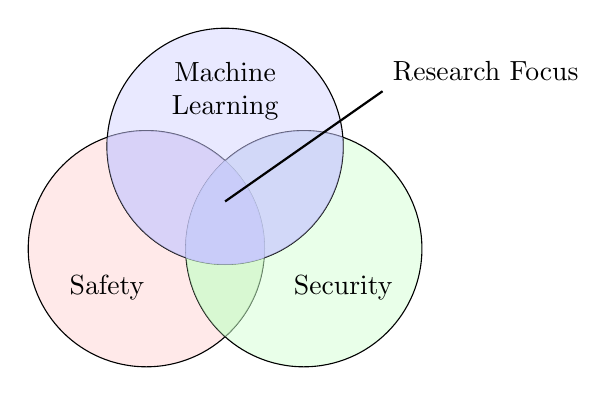
\begin{tikzpicture}
    % Colors with opacity
    \definecolor{color1}{RGB}{255, 200, 200}
    \definecolor{color2}{RGB}{200, 255, 200}
    \definecolor{color3}{RGB}{200, 200, 255}
    
    % Circles
    \draw[fill=color1, fill opacity=0.4] (0,0) circle (1.5cm);
    \draw[fill=color2, fill opacity=0.4] (2,0) circle (1.5cm);
    \draw[fill=color3, fill opacity=0.4] (1, 1.3) circle (1.5cm);
    
    % Darker intersections
    \begin{scope}
      \clip (0,0) circle (1.5cm);
      \fill[color2, opacity=0.5] (2,0) circle (1.5cm);
    \end{scope}
    
    \begin{scope}
      \clip (0,0) circle (1.5cm);
      \fill[color3, opacity=0.5] (1,1.3) circle (1.5cm);
    \end{scope}
    
    \begin{scope}
      \clip (2,0) circle (1.5cm);
      \fill[color3, opacity=0.5] (1,1.3) circle (1.5cm);
    \end{scope}
    
    \begin{scope}
      \clip (0,0) circle (1.5cm);
      \clip (2,0) circle (1.5cm);
      \fill[color3, opacity=0.5] (1,1.3) circle (1.5cm);
    \end{scope}
  
    % Annotations within the circles
    \node at (-0.5, -0.5) {Safety};
    \node at (2.5, -0.5) {Security};
    \node at (1, 2) {\begin{tabular}{c} Machine \\ Learning \end{tabular}};
    
    % Line pointing to "Research Focus"
  \draw[-, thick] (1, 0.6) -- (3, 2) node[above right] {Research Focus};
  
  \end{tikzpicture}
  \end{center}
\end{frame}


\begin{frame}
  \frametitle{Outline}
  \tableofcontents
\end{frame}

\section{Introduction}


\begin{frame}
  \frametitle{Embedded Systems}
  
  \begin{center}
    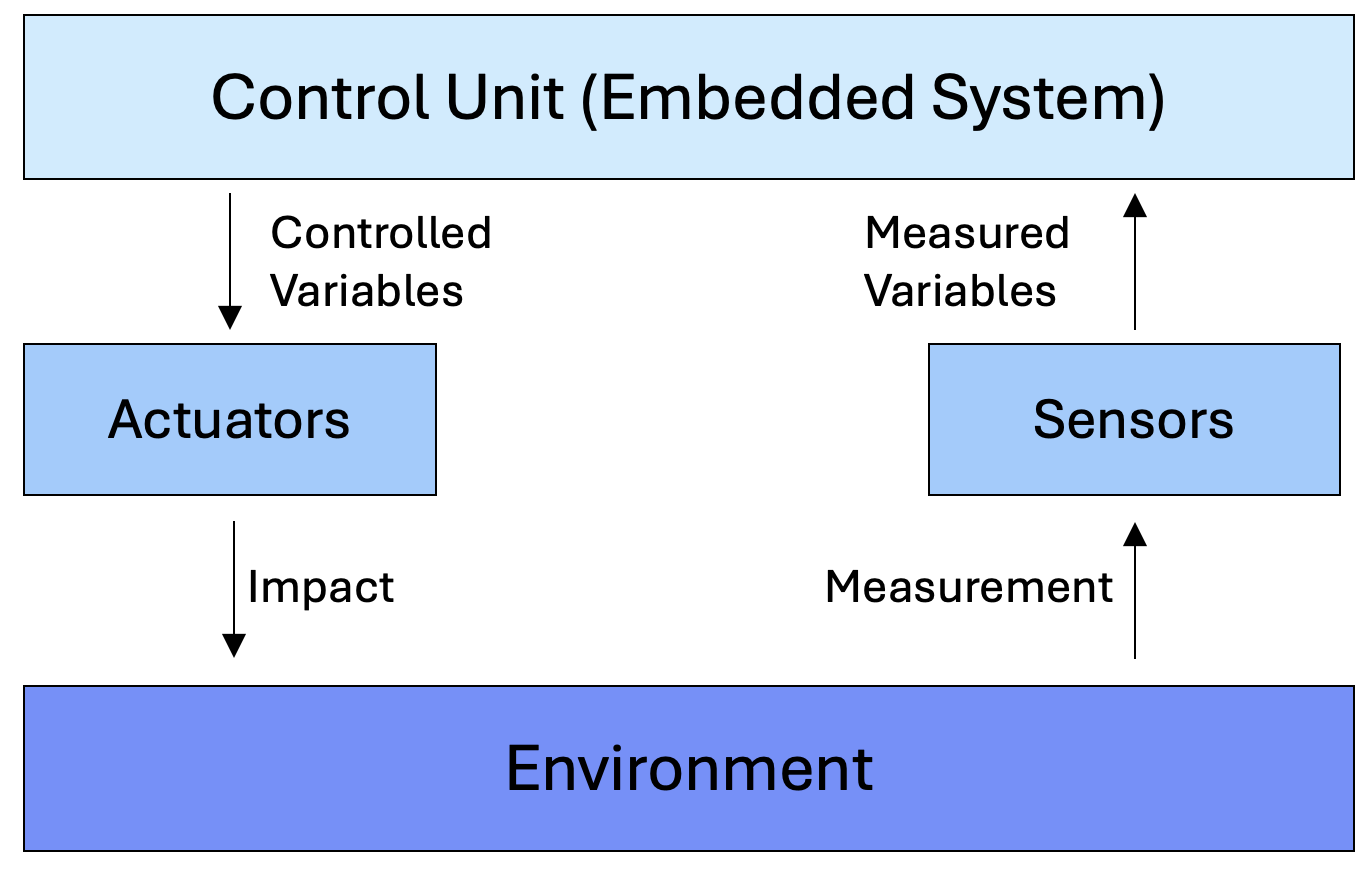
\includegraphics[width=\linewidth]{images/embedded_system.png}
  \end{center}
  
  \end{frame}

  \begin{frame}{Why formal verification?}
  
  \end{frame}

\section{First-order logic}
\begin{frame}{Language of first-order logic}
  
    A language $\mathscr{L}$ of first-order logic consists of the following components:
    \begin{itemize}
    \item Variable symbols: $x_1, x_2, \ldots$
    \item For each $n\in\mathbb{N}$, a set of $n$-ary function symbols: $f_0, f_1, \ldots$ The 0-ary function symbols are called constant symbols.
    \item For each $n\in\mathbb{N}$, a set of $n$-ary predicate symbols: $p_0, p_1, \ldots$ The 0-ary predicate symbols are the constants $\top$ (for \textbf{true}) and $\bot$ (for \textbf{false}).
    \item special symbols: $\neg$ (negation), $\wedge$ (conjunction), $\vee$ (disjunction), $\rightarrow$ (implication), $\leftrightarrow$ (equivalence), $\forall$ (universal quantification), $\exists$ (existential quantification), and parentheses.
  \end{itemize}

  \end{frame}

  \begin{frame}{Terms}

    The set of terms of $\mathscr{L}$ is defined inductively as follows:
    \begin{itemize}
    \item Each variable is a term.
    \item If $t_1, \ldots, t_n$ are terms and $f$ is an $n$-ary function symbol, then if $f(t_1, \ldots, t_n)$ is a term.
  \end{itemize}
  \end{frame}

  \begin{frame}{Variables in terms}
    We define a function $var: \text{Terms}\rightarrow\text{Variables}$ that maps each term to the set of variables occurring in it. The function is defined as follows:
    \begin{itemize}
    \item $var(x) = \{x\}$ for each variable $x$.
    \item $var(f(t_1, \ldots, t_n)) = var(t_1)\cup\ldots\cup var(t_n)$.
  \end{itemize}
  \end{frame}
  \begin{frame}{Formulas}
    The set of formulas of $\mathscr{L}$ is defined inductively as follows:
    \begin{itemize}
    \item If $t_1, \ldots, t_n$ are terms and $p$ is an $n$-ary predicate symbol, then if $p(t_1, \ldots, t_n)$ is a formula.
    \item If $\varphi$ is a formula, then if $\neg\varphi$ is a formula.
    \item If $\varphi_1$ and $\varphi_2$ are formulas, then if $\varphi_1\wedge\varphi_2$, $\varphi_1\vee\varphi_2$, $\varphi_1\rightarrow\varphi_2$, and $\varphi_1\leftrightarrow\varphi_2$ are formulas.
    \item If $\varphi$ is a formula and $x$ is a variable, then if $\forall x.\varphi$ and $\exists x.\varphi$ are formulas.
  \end{itemize}
  An example of a formula is $\forall x. \exists y. p(x, y) \rightarrow \neg q(y)$.
  \end{frame}

  \begin{frame}{Interpretations}
    
    An interpretation $\mathcal{M}$ of $\mathscr{L}$ consists of the following components:
    \begin{itemize}
    \item A non-empty set $D$ called the domain of $\mathcal{M}$.
    \item For each $n$-ary function symbol $f$ of $\mathscr{L}$, a function $f^{\mathcal{M}}: D^n\rightarrow D$.
    \item For each $n$-ary predicate symbol $p$ of $\mathscr{L}$, a relation $p^{\mathcal{M}}\subseteq D^n$.
  \end{itemize}
  \end{frame}

  \begin{frame}{Interpretations of Terms}
    Let $\mathcal{M}$ be an interpretation for our first-order language. 
    An assignment $\sigma$ of values to variables, i.e., $\sigma: Variables\rightarrow D$. 
    
    The value of a term $t$ under $\sigma$ is denoted by $t^{\mathcal{M}}[\sigma]$ and defined as follows:
    \begin{itemize}
    \item If $t=x$ for a variable $x$, then $t^{\mathcal{M}}[\sigma]=\sigma(x)$.
    \item If $t=f(t_1, \ldots, t_n)$, then $t^{\mathcal{M}}[\sigma]=f^{\mathcal{M}}(t_1^{\mathcal{M}}[\sigma], \ldots, t_n^{\mathcal{M}}[\sigma])$.
    \end{itemize}
  \end{frame}
  \begin{frame}{Validity of Formulas under Interpretations}
    We say an assignment $\sigma$ satisfies a formula $\varphi$ under an interpretation $\mathcal{M}$, denoted by $\mathcal{M}, \sigma\models\varphi$, iff the following conditions hold:
    \begin{itemize}
    \item $\varphi=p(t_1, \ldots, t_n)$, then if $(t_1^{\mathcal{M}}[\sigma], \ldots, t_n^{\mathcal{M}}[\sigma])\in p^{\mathcal{M}}$.
    \item $\varphi=\neg\psi$, then if $\mathcal{M}, \sigma\not\models\psi$.
    \item $\varphi=\psi_1\vee\psi_2$, then if $\mathcal{M}, \sigma\models\psi_1$ or $\mathcal{M}, \sigma\models\psi_2$.
    \item $\varphi=\psi_1\wedge\psi_2$, then if $\mathcal{M}, \sigma\models\psi_1$ and $\mathcal{M}, \sigma\models\psi_2$.
    \item $\varphi=\psi_1\rightarrow\psi_2$, then if $\mathcal{M}, \sigma\models\psi_1$ implies $\mathcal{M}, \sigma\models\psi_2$.
    \item $\varphi=\psi_1\leftrightarrow\psi_2$, then if $\mathcal{M}, \sigma\models\psi_1$ if and only if $\mathcal{M}, \sigma\models\psi_2$.
    \item $\varphi=\forall x.\psi$, then if $\mathcal{M}, \sigma[x\mapsto d]\models\psi$ for all $d\in D$.
    \item $\varphi=\exists x.\psi$, then if $\mathcal{M}, \sigma[x\mapsto d]\models\psi$ for some $d\in D$.
    \end{itemize}
    A formula $\varphi$ is satisfiable if there exists an interpretation $\mathcal{M}$ and an assignment $\sigma$ such that $\mathcal{M}, \sigma\models\varphi$.
  \end{frame}


  \begin{frame}{Models}
    An interpretation $\mathcal{M}$ is a model of a formula $\varphi$, denoted by $\mathcal{M}\models\varphi$, if for all assignments $\sigma$, $\mathcal{M}, \sigma\models\varphi$.
    
    \vspace*{0.5cm}
    A formula is satisfiable if it has a model, i.e., if there exists an interpretation $\mathcal{M}$ such that $\mathcal{M}\models\varphi$.
    
    
  \end{frame}
 

  \begin{frame}{Validity}
    A formula $\varphi$ is valid if for all interpretations $\mathcal{M}$ and all assignments $\sigma$, $\mathcal{M}, \sigma\models\varphi$.
    
    We write $\models\varphi$ to denote that $\varphi$ is valid.
  \end{frame}

  \begin{frame}{Free Variables in Fomulas}
    The set of free variables of a formula $\varphi$, denoted by $FV(\varphi)$, is defined inductively as follows:
    \begin{itemize}
    \item $FV(p(t_1, \ldots, t_n))=var(t_1)\cup\ldots\cup var(t_n)$.
    \item $FV(\neg\psi)=FV(\psi)$.
    \item $FV(\psi_1\wedge\psi_2)=FV(\psi_1)\cup FV(\psi_2)$.
    \item $FV(\psi_1\vee\psi_2)=FV(\psi_1)\cup FV(\psi_2)$.
    \item $FV(\psi_1\rightarrow\psi_2)=FV(\psi_1)\cup FV(\psi_2)$.
    \item $FV(\forall x.\psi)=FV(\psi)\setminus\{x\}$.
    \item $FV(\exists x.\psi)=FV(\psi)\setminus\{x\}$.
    \end{itemize}
  \end{frame}

  \begin{frame}{Term Substitution}
    Let $\varphi$ be a formula, $x$ a variable, and $t$ a term. The formula $\varphi[t/x]$ is obtained by replacing all occurrences of $x$ in $\varphi$ by $t$. The substitution is defined inductively as follows:
    \begin{itemize}
    \item $(p(t_1, \ldots, t_n))[t/x]=p(t_1[t/x], \ldots, t_n[t/x])$.
    \item $(\neg\psi)[t/x]=\neg\psi[t/x]$.
    \item $(\psi_1\wedge\psi_2)[t/x]=\psi_1[t.x]\wedge\psi_2[t/x]$.
    \item $(\psi_1\vee\psi_2)[t/x]=\psi_1[t/x]\vee\psi_2[t/x]$.
    \item $(\psi_1\rightarrow\psi_2)[t/x]=\psi_1[t/x]\rightarrow\psi_2[t/x]$.
    \item   $(\forall y.\psi)[t/x]=\forall y.\psi[t/x]$ if $x\in FV(t)$.
    \item $(\exists y.\psi)[t/x]=\exists y.\psi[t/x]$ if $x\in FV(t)$.
    \item $(\forall x.\psi)[t/x]=\forall x.\psi$.
    \item $(\exists x.\psi)[t/x]=\exists x.\psi$.
    \end{itemize}

    So, $\varphi[t/x]$ represents the formular obtained by substituting every \textbf{free} occurrence of the variable $x$ in $\varphi$ by the term $t$.
  \end{frame}
    
  \begin{frame}{Calculus}
    A calculus is a mechanism to prove formulas by applying rules.

    A rule of a calculus has the form $\frac{\varphi_1, \ldots, \varphi_n}{\psi}$, where $\varphi_1, \ldots, \varphi_n$ are premises and $\psi$ is the conclusion. The rule states that if $\varphi_1, \ldots, \varphi_n$ are derivable, then $\psi$ is derivable.

    We denote that a formula can be proved by a calculus by $\vdash\varphi$.
  \end{frame}
% ****************************



% \begin{frame}
%   \frametitle{Some Natural Deduction Rules}
%   \begin{columns}
  
%   \column{0.5\textwidth}
%   \textbf{Conjunction Introduction ($\land$ I)}
%   \begin{prooftree}
%     \AxiomC{$A$}
%     \AxiomC{$B$}
%     \RightLabel{$\land$ I}
%     \BinaryInfC{$A \land B$}
%   \end{prooftree}
  
%   \vspace{10pt}
  
%   \textbf{Conjunction Elimination ($\land$ E)}
%   \begin{prooftree}
%     \AxiomC{$A \land B$}
%     \RightLabel{$\land$ E$_1$}
%     \UnaryInfC{$A$}
%   \end{prooftree}
%   \begin{prooftree}
%     \AxiomC{$A \land B$}
%     \RightLabel{$\land$ E$_2$}
%     \UnaryInfC{$B$}
%   \end{prooftree}
  
%   \column{0.5\textwidth}
%   \textbf{Disjunction Introduction ($\lor$ I)}
%   \begin{prooftree}
%     \AxiomC{$A$}
%     \RightLabel{$\lor$ I$_1$}
%     \UnaryInfC{$A \lor B$}
%   \end{prooftree}
%   \begin{prooftree}
%     \AxiomC{$B$}
%     \RightLabel{$\lor$ I$_2$}
%     \UnaryInfC{$A \lor B$}
%   \end{prooftree}
  
%   \vspace{10pt}
  
%   \textbf{Disjunction Elimination ($\lor$ E)}
%   \begin{prooftree}
%     \AxiomC{$A \lor B$}
%     \AxiomC{$[A]$}
%     \noLine
%     \UnaryInfC{$\vdots$}
%     \noLine
%     \UnaryInfC{$C$}
%     \AxiomC{$[B]$}
%     \noLine
%     \UnaryInfC{$\vdots$}
%     \noLine
%     \UnaryInfC{$C$}
%     \RightLabel{$\lor$ E}
%     \TrinaryInfC{$C$}
%   \end{prooftree}
  
%   \end{columns}
%   \end{frame}
  
  % \begin{frame}
  % \frametitle{Natural Deduction Rules (cont.)}
  % \begin{columns}
  
  % \column{0.5\textwidth}
  % \textbf{Implication Introduction ($\implies$ I)}
  % \begin{prooftree}
  %   \AxiomC{$[A]$}
  %   \noLine
  %   \UnaryInfC{$\vdots$}
  %   \noLine
  %   \UnaryInfC{$B$}
  %   \RightLabel{$\implies$ I}
  %   \UnaryInfC{$A \implies B$}
  % \end{prooftree}
  
  % \vspace{10pt}
  
  % \textbf{Implication Elimination (Modus Ponens, $\implies$ E)}
  % \begin{prooftree}
  %   \AxiomC{$A \implies B$}
  %   \AxiomC{$A$}
  %   \RightLabel{$\implies$ E}
  %   \BinaryInfC{$B$}
  % \end{prooftree}
  
  % \column{0.5\textwidth}
  % \textbf{Negation Introduction ($\neg$ I)}
  % \begin{prooftree}
  %   \AxiomC{$[A]$}
  %   \noLine
  %   \UnaryInfC{$\vdots$}
  %   \noLine
  %   \UnaryInfC{$\bot$}
  %   \RightLabel{$\neg$ I}
  %   \UnaryInfC{$\neg A$}
  % \end{prooftree}
  
  % \vspace{10pt}
  
  % \textbf{Negation Elimination ($\neg$ E)}
  % \begin{prooftree}
  %   \AxiomC{$A$}
  %   \AxiomC{$\neg A$}
  %   \RightLabel{$\neg$ E}
  %   \BinaryInfC{$\bot$}
  % \end{prooftree}
  
  % \end{columns}
  % \end{frame}
  
  % \begin{frame}
  % \frametitle{Natural Deduction Rules (cont.)}
  % \begin{columns}
  
  % \column{0.5\textwidth}
  % \textbf{Double Negation Elimination ($\neg\neg$ E)}
  % \begin{prooftree}
  %   \AxiomC{$\neg\neg A$}
  %   \RightLabel{$\neg\neg$ E}
  %   \UnaryInfC{$A$}
  % \end{prooftree}
  
  % \vspace{10pt}
  
  % \textbf{Biconditional Introduction ($\iff$ I)}
  % \begin{prooftree}
  %   \AxiomC{$A \implies B$}
  %   \AxiomC{$B \implies A$}
  %   \RightLabel{$\iff$ I}
  %   \BinaryInfC{$A \iff B$}
  % \end{prooftree}
  
  % \column{0.5\textwidth}
  % \textbf{Biconditional Elimination ($\iff$ E)}
  % \begin{prooftree}
  %   \AxiomC{$A \iff B$}
  %   \RightLabel{$\iff$ E$_1$}
  %   \UnaryInfC{$A \implies B$}
  % \end{prooftree}
  % \begin{prooftree}
  %   \AxiomC{$A \iff B$}
  %   \RightLabel{$\iff$ E$_2$}
  %   \UnaryInfC{$B \implies A$}
  % \end{prooftree}
  
  % \end{columns}
  % \end{frame}

  % \begin{frame}
  %   \frametitle{Some Natural Deduction Rules: Quantifiers}
  %   \begin{columns}
    
  %   \column{0.5\textwidth}
  %   \textbf{Universal Introduction ($\forall$ I)}
  %   \begin{prooftree}
  %     \AxiomC{$[x]$}
  %     \noLine
  %     \UnaryInfC{$\vdots$}
  %     \noLine
  %     \UnaryInfC{$A(x)$}
  %     \RightLabel{$\forall$ I}
  %     \UnaryInfC{$\forall x \, A(x)$}
  %   \end{prooftree}
    
  %   \vspace{10pt}
    
  %   \textbf{Universal Elimination ($\forall$ E)}
  %   \begin{prooftree}
  %     \AxiomC{$\forall x \, A(x)$}
  %     \RightLabel{$\forall$ E}
  %     \UnaryInfC{$A(t)$}
  %   \end{prooftree}
    
  %   \column{0.5\textwidth}
  %   \textbf{Existential Introduction ($\exists$ I)}
  %   \begin{prooftree}
  %     \AxiomC{$A(t)$}
  %     \RightLabel{$\exists$ I}
  %     \UnaryInfC{$\exists x \, A(x)$}
  %   \end{prooftree}
    
  %   \vspace{10pt}
    
  %   \textbf{Existential Elimination ($\exists$ E)}
  %   \begin{prooftree}
  %     \AxiomC{$\exists x \, A(x)$}
  %     \AxiomC{$[A(x)]$}
  %     \noLine
  %     \UnaryInfC{$\vdots$}
  %     \noLine
  %     \UnaryInfC{$C$}
  %     \RightLabel{$\exists$ E}
  %     \BinaryInfC{$C$}
  %   \end{prooftree}
    
  %   \end{columns}
  %   \end{frame}

    % \begin{frame}
    %   \frametitle{Example Deduction: \(\forall x (P(x) \rightarrow Q(x)), \forall x P(x) \vdash \forall x Q(x)\)}
      
    %   \begin{prooftree}
    %     \AxiomC{}
    %     \RightLabel{Premise}
    %     \UnaryInfC{$\forall x (P(x) \rightarrow Q(x))$}
    %     \AxiomC{}
    %     \RightLabel{Premise}
    %     \UnaryInfC{$\forall x P(x)$}
    %     \RightLabel{$\forall$ E}
    %     \UnaryInfC{$P(a)$}
    %     \RightLabel{$\forall$ E}
    %     \UnaryInfC{$P(a) \rightarrow Q(a)$}
    %     \RightLabel{$\rightarrow$ E}
    %     \BinaryInfC{$Q(a)$}
    %     \RightLabel{$\forall$ I}
    %     \UnaryInfC{$\forall x Q(x)$}
    %   \end{prooftree}
      
      % \end{frame}
%*****************

\begin{frame}{Sequent Calculus}
  

  In sequent calculus, we have sequences $\Gamma\vdash\Delta$, where $\Gamma$ and $\Delta$ are sets of formulas.
  \vspace*{1cm}

  The interpretation is that if all formulas in $\Gamma$ are true, then at least one formula in $\Delta$ is true.
  \end{frame}
  
  
    \begin{frame}{Sequent Calculus Rules}
      \begin{columns}
        \column{0.5\textwidth}
      \begin{prooftree}
        \AxiomC{-}
        \RightLabel{Taut}
        \UnaryInfC{$\Gamma, \varphi \Rightarrow \varphi, \Delta$}
      \end{prooftree}
      \column{0.5\textwidth}
      \begin{prooftree}
        \AxiomC{$\Gamma\Rightarrow\Delta,\varphi\hspace*{0.5cm}\varphi,\Pi\Rightarrow\Lambda$}
        \RightLabel{Cut}
        \UnaryInfC{$\Gamma,\Pi \Rightarrow\Delta,\Lambda$}
      \end{prooftree}
    \end{columns}

      \begin{columns}
    
      \column{0.5\textwidth}
      \begin{prooftree}
        \AxiomC{-}
        \RightLabel{$\bot \Rightarrow$}
        \UnaryInfC{$\Gamma, \bot \Rightarrow \Delta$}
      \end{prooftree}
      \column{0.5\textwidth}
      \begin{prooftree}
        \AxiomC{-}
        \RightLabel{$\Rightarrow\top$}
        \UnaryInfC{$\Gamma\Rightarrow \Delta,\top$}
      \end{prooftree}
    \end{columns}


    \begin{columns}
      \column{0.5\textwidth}
    \begin{prooftree}
      \AxiomC{$\Gamma\Rightarrow\Delta$}
      \RightLabel{Weakening left}
      \UnaryInfC{$\varphi,\Gamma\Rightarrow\Delta$}
    \end{prooftree}
    \column{0.5\textwidth}
    \begin{prooftree}
      \AxiomC{$\Gamma\Rightarrow\Delta$}
      \RightLabel{Weakening right}
      \UnaryInfC{$\Gamma\Rightarrow\Delta,\varphi$}
    \end{prooftree}
  \end{columns}

  \begin{columns}
    \column{0.5\textwidth}
  \begin{prooftree}
    \AxiomC{$\varphi,\varphi,\Gamma\Rightarrow\Delta$}
    \RightLabel{Contraction left}
    \UnaryInfC{$\varphi,\Gamma\Rightarrow\Delta$}
  \end{prooftree}
  \column{0.5\textwidth}
  \begin{prooftree}
    \AxiomC{$\Gamma\Rightarrow\Delta,\varphi,\varphi$}
    \RightLabel{Contraction right}
    \UnaryInfC{$\Gamma\Rightarrow\Delta,\varphi$}
  \end{prooftree}
\end{columns}

\begin{columns}
  \column{0.5\textwidth}
\begin{prooftree}
  \AxiomC{$\Gamma,\varphi,\psi,\Pi\Rightarrow\Delta$}
  \RightLabel{Exchange left}
  \UnaryInfC{$\Gamma,\psi,\varphi,\Pi\Rightarrow\Delta$}
\end{prooftree}
\column{0.5\textwidth}
\begin{prooftree}
  \AxiomC{$\Gamma\Rightarrow\Delta,\varphi,\psi,\Lambda$}
  \RightLabel{Exchange right}
  \UnaryInfC{$\Gamma\Rightarrow\Delta,\psi,\varphi,\Lambda$}
\end{prooftree}
\end{columns}

  
  \end{frame}
  \begin{frame}{Sequent Calculus Rules}

    \begin{columns}
  
    \column{0.5\textwidth}
    \begin{prooftree}
      \AxiomC{-}
      \RightLabel{$\bot \Rightarrow$}
      \UnaryInfC{$\Gamma, \bot \Rightarrow \Delta$}
    \end{prooftree}
    \column{0.5\textwidth}
    \begin{prooftree}
      \AxiomC{-}
      \RightLabel{$\Rightarrow\top$}
      \UnaryInfC{$\Gamma\Rightarrow \Delta,\top$}
    \end{prooftree}
  \end{columns}


    \begin{columns}
    
      \column{0.5\textwidth}
      \begin{prooftree}
        \AxiomC{$\Gamma\Rightarrow\Delta,\varphi$}
        \RightLabel{$\neg\Rightarrow$}
        \UnaryInfC{$\Gamma,\neg \varphi\Rightarrow \Delta$}
      \end{prooftree}
      \column{0.5\textwidth}
      \begin{prooftree}
        \AxiomC{$\Gamma,\varphi\Rightarrow\Delta$}
        \RightLabel{$\Rightarrow\neg$}
        \UnaryInfC{$\Gamma\Rightarrow \Delta,\neg\varphi$}
      \end{prooftree}
      \end{columns}
      

      \begin{columns}
    
        \column{0.5\textwidth}
        \begin{prooftree}
          \AxiomC{$\Gamma,\varphi\Rightarrow\Delta \hspace*{0.5cm} \Gamma,\psi\Rightarrow \Delta$}
          \RightLabel{$\vee\Rightarrow$}
          \UnaryInfC{$\Gamma,\varphi\vee \psi\Rightarrow \Delta$}
        \end{prooftree}
        \column{0.5\textwidth}
        \begin{prooftree}
          \AxiomC{$\Gamma\Rightarrow\Delta,\varphi,\psi$}
          \RightLabel{$\Rightarrow\vee$}
          \UnaryInfC{$\Gamma\Rightarrow \Delta,\varphi\vee \psi$}
        \end{prooftree}
        \end{columns}

        \begin{columns}
    
          \column{0.5\textwidth}
          \begin{prooftree}
            \AxiomC{$\Gamma,\varphi,\psi\Rightarrow\Delta$}
            \RightLabel{$\wedge\Rightarrow$}
            \UnaryInfC{$\Gamma,\varphi\wedge \psi\Rightarrow \Delta$}
          \end{prooftree}
          \column{0.5\textwidth}
          \begin{prooftree}
            \AxiomC{$\Gamma\Rightarrow\Delta,\varphi \hspace*{0.5cm}\Gamma\Rightarrow\Delta,\psi$}
            \RightLabel{$\Rightarrow\wedge$}
            \UnaryInfC{$\Gamma\Rightarrow \Delta,\varphi\wedge \psi$}
          \end{prooftree}
          \end{columns}


          \begin{columns}
    
            \column{0.5\textwidth}
            \begin{prooftree}
              \AxiomC{$\Gamma\Rightarrow\Delta,\varphi\hspace*{0.5cm}\psi,\Pi\Rightarrow\Lambda$}
              \RightLabel{$\to\Rightarrow$}
              \UnaryInfC{$\varphi\to\psi,\Gamma,\Pi\Rightarrow \Delta,\Lambda$}
            \end{prooftree}
            \column{0.5\textwidth}
            \begin{prooftree}
              \AxiomC{$\Gamma,\varphi\Rightarrow\Delta,\psi$}
              \RightLabel{$\Rightarrow\to$}
              \UnaryInfC{$\Gamma\Rightarrow \Delta,\varphi\to \psi$}
            \end{prooftree}
            \end{columns}



      \end{frame}

      \begin{frame}{Sequent Calculus Rules}
        \begin{columns}
    
          \column{0.5\textwidth}
          \begin{prooftree}
            \AxiomC{$\Gamma,\varphi[t/x]\Rightarrow\Delta$}
            \RightLabel{$\forall\Rightarrow$}
            \UnaryInfC{$\Gamma,\forall x.\varphi(x)\Rightarrow\Delta$}
          \end{prooftree}
          \column{0.5\textwidth}
          \begin{prooftree}
            \AxiomC{$\Gamma\Rightarrow\Delta,\varphi[y/x]$}
            \RightLabel{$\Rightarrow\forall$}
            \UnaryInfC{$\Gamma\Rightarrow\Delta,\forall x.\varphi(x)$}
          \end{prooftree}
          \end{columns}

          
          \begin{columns}
    
            \column{0.5\textwidth}
            \begin{prooftree}
              \AxiomC{$\Gamma,\varphi[y/x]\Rightarrow\Delta$}
              \RightLabel{$\exists\Rightarrow$}
              \UnaryInfC{$\Gamma,\exists x.\varphi(x)\Rightarrow\Delta$}
            \end{prooftree}
            \column{0.5\textwidth}
            \begin{prooftree}
              \AxiomC{$\Gamma\Rightarrow\Delta,\exists x.\varphi(x),\varphi[t/x]$}
              \RightLabel{$\Rightarrow\exists$}
              \UnaryInfC{$\Gamma\Rightarrow\Delta,\exists x.\varphi(x)$}
            \end{prooftree}
            \end{columns}

            \vspace{0.5cm}

            In the quantifier rules, $t$ is a term, and $y$ is a 'fresh' variable, i.e., a variable that does not occur in $\Gamma$, $\Delta$, or $\varphi$. 
            
            Alternatively, the rules can also be stated in the form
        
            \begin{prooftree}
              \AxiomC{$\Gamma\Rightarrow\Delta,\varphi$}
              \RightLabel{$\Rightarrow\forall$}
              \UnaryInfC{$\Gamma\Rightarrow\Delta,\forall x.\varphi(x)$}
            \end{prooftree}

            Here, it must be guaranteed that $x$ is not free in any formula in $\Gamma$ or $\Delta$. The existential formula can be handled similarly.
      \end{frame}
      
    %   \begin{frame}
    %   \frametitle{Sequent Calculus Rules: Logical Connectives (cont.)}
    %   \begin{columns}
      
    %   \column{0.5\textwidth}
    %   \textbf{Implication Rules ($\implies$)}
    %   \begin{prooftree}
    %     \AxiomC{$\Gamma, A \vdash B$}
    %     \RightLabel{$\implies$ R}
    %     \UnaryInfC{$\Gamma \vdash A \implies B$}
    %   \end{prooftree}
      
    %   \begin{prooftree}
    %     \AxiomC{$\Gamma \vdash A$}
    %     \AxiomC{$\Gamma, B \vdash \Delta$}
    %     \RightLabel{$\implies$ L}
    %     \BinaryInfC{$\Gamma, A \implies B \vdash \Delta$}
    %   \end{prooftree}
      
    %   \column{0.5\textwidth}
    %   \textbf{Negation Rules ($\neg$)}
    %   \begin{prooftree}
    %     \AxiomC{$\Gamma, A \vdash \Delta$}
    %     \RightLabel{$\neg$ R}
    %     \UnaryInfC{$\Gamma \vdash \neg A$}
    %   \end{prooftree}
      
    %   \begin{prooftree}
    %     \AxiomC{$\Gamma \vdash A$}
    %     \RightLabel{$\neg$ L}
    %     \UnaryInfC{$\Gamma, \neg A \vdash \Delta$}
    %   \end{prooftree}
      
    %   \end{columns}
    %   \end{frame}
      
    %   \begin{frame}
    %   \frametitle{Sequent Calculus Rules: Quantifiers}
    %   \begin{columns}
      
    %   \column{0.5\textwidth}
    %   \textbf{Universal Quantifier ($\forall$)}
    %   \begin{prooftree}
    %     \AxiomC{$\Gamma \vdash A(x)$}
    %     \RightLabel{$\forall$ R}
    %     \UnaryInfC{$\Gamma \vdash \forall x \, A(x)$}
    %   \end{prooftree}
      
    %   \begin{prooftree}
    %     \AxiomC{$\Gamma, A(t) \vdash \Delta$}
    %     \RightLabel{$\forall$ L}
    %     \UnaryInfC{$\Gamma, \forall x \, A(x) \vdash \Delta$}
    %   \end{prooftree}
      
    %   \column{0.5\textwidth}
    %   \textbf{Existential Quantifier ($\exists$)}
    %   \begin{prooftree}
    %     \AxiomC{$\Gamma \vdash A(t)$}
    %     \RightLabel{$\exists$ R}
    %     \UnaryInfC{$\Gamma \vdash \exists x \, A(x)$}
    %   \end{prooftree}
      
    %   \begin{prooftree}
    %     \AxiomC{$\Gamma, A(x) \vdash \Delta$}
    %     \RightLabel{$\exists$ L}
    %     \UnaryInfC{$\Gamma, \exists x \, A(x) \vdash \Delta$}
    %   \end{prooftree}
      
    %   \end{columns}
    %   \end{frame}
      
    %   \begin{frame}
    %   \frametitle{Sequent Calculus Rules: Structural Rules}
    %   \begin{columns}
      
    %   \column{0.5\textwidth}
    %   \textbf{Weakening}
    %   \begin{prooftree}
    %     \AxiomC{$\Gamma \vdash \Delta$}
    %     \RightLabel{WL}
    %     \UnaryInfC{$\Gamma, A \vdash \Delta$}
    %   \end{prooftree}
    %   \begin{prooftree}
    %     \AxiomC{$\Gamma \vdash \Delta$}
    %     \RightLabel{WR}
    %     \UnaryInfC{$\Gamma \vdash \Delta, A$}
    %   \end{prooftree}
      
    %   \vspace{10pt}
      
    %   \textbf{Contraction}
    %   \begin{prooftree}
    %     \AxiomC{$\Gamma, A, A \vdash \Delta$}
    %     \RightLabel{CL}
    %     \UnaryInfC{$\Gamma, A \vdash \Delta$}
    %   \end{prooftree}
    %   \begin{prooftree}
    %     \AxiomC{$\Gamma \vdash \Delta, A, A$}
    %     \RightLabel{CR}
    %     \UnaryInfC{$\Gamma \vdash \Delta, A$}
    %   \end{prooftree}
      
    %   \column{0.5\textwidth}
    %   \textbf{Exchange}
    %   \begin{prooftree}
    %     \AxiomC{$\Gamma, A, B, \Sigma \vdash \Delta$}
    %     \RightLabel{EL}
    %     \UnaryInfC{$\Gamma, B, A, \Sigma \vdash \Delta$}
    %   \end{prooftree}
    %   \begin{prooftree}
    %     \AxiomC{$\Gamma \vdash \Delta, A, B, \Pi$}
    %     \RightLabel{ER}
    %     \UnaryInfC{$\Gamma \vdash \Delta, B, A, \Pi$}
    %   \end{prooftree}
      
    %   \vspace{10pt}
      
    %   \textbf{Cut}
    %   \begin{prooftree}
    %     \AxiomC{$\Gamma \vdash A, \Delta$}
    %     \AxiomC{$\Gamma, A \vdash \Delta$}
    %     \RightLabel{Cut}
    %     \BinaryInfC{$\Gamma \vdash \Delta$}
    %   \end{prooftree}
      
    %   \end{columns}
    %   \end{frame}

      

        \begin{frame}
          \frametitle{Example Deduction: \(\forall x.(P(x)\wedge Q\Rightarrow\forall x.P(x)\)}
          
          \begin{prooftree}
            \AxiomC{}
            \RightLabel{Taut}
            \UnaryInfC{$P(x),Q\Rightarrow P(x)$}
          
            
            \RightLabel{$\wedge\Rightarrow$ }
            \UnaryInfC{$P(x)\wedge Q\Rightarrow P(x)$}
          
            \RightLabel{$\forall\Rightarrow$}
            \UnaryInfC{$\forall x.(P(x\wedge Q)\Rightarrow P(x))$}
          
            \RightLabel{$\Rightarrow\forall$}
            \UnaryInfC{$\forall x.(P(x)\wedge Q)\Rightarrow\forall x.P(x)$}
          
          \end{prooftree}
          \vspace*{0.5cm}
          Here, $\forall\Rightarrow$ uses $[x/x]$ as replacement, i.e., just the same free variable is taken.
          \end{frame}


          \begin{frame}
            \frametitle{Example Deduction: \(\forall x.(A\to B)\Rightarrow A\to\forall x.B\)}
            
            \begin{prooftree}
              \AxiomC{}
              \RightLabel{Taut}
              \UnaryInfC{$A\Rightarrow A,B$}

              \AxiomC{}
              \RightLabel{Taut}
              \UnaryInfC{$A,B\Rightarrow B$}
            
              
              
              \RightLabel{$\to\Rightarrow$ }
              \BinaryInfC{$A,A\to B\Rightarrow B$}
            
             
              \RightLabel{$\forall\Rightarrow$}
              \UnaryInfC{$A,\forall x.(A\to B)\Rightarrow B$}
            
              \RightLabel{$\Rightarrow\forall$}
              \UnaryInfC{$A,\forall x.(A\to B)\Rightarrow \forall x.B$}
              \RightLabel{$\Rightarrow\to$}
              \UnaryInfC{$\forall x.(A\to B)\Rightarrow A\to \forall x.B$}
              
            
            \end{prooftree}
            \vspace*{0.5cm}
            Here, the application of $\Rightarrow\forall$ requires that $x$ is not free in $A$.

            \end{frame}

            \begin{frame}
              \frametitle{Example of a Failing Deduction: \(\exists x.P(x)\wedge \exists x.Q(x)\Rightarrow\exists x.(P(x)\wedge Q(x))\)}
              
              \begin{prooftree}
                \AxiomC{$P(x),Q(y)\Rightarrow P(x)\wedge Q(x)$}
                \RightLabel{$\Rightarrow\exists$}
                \UnaryInfC{$P(x),Q(y)\Rightarrow\exists x.(P(x)\wedge Q(x))$}
                \RightLabel{$\exists\Rightarrow$}
                \UnaryInfC{$P(x),\exists x.Q(x)\Rightarrow\exists x.(P(x)\wedge Q(x))$}
                \RightLabel{$\exists\Rightarrow$}
                \UnaryInfC{$\exists x.P(x),\exists x.Q(x)\Rightarrow\exists x.(P(x)\wedge Q(x))$}
                \RightLabel{$\wedge\Rightarrow$}
                \UnaryInfC{$\exists x.P(x)\wedge \exists x.Q(x)\Rightarrow\exists x.(P(x)\wedge Q(x))$}
              
              \end{prooftree}
              \vspace*{0.5cm}
              Here, the deduction fails because the variable $x$ is not fresh in the application of $\exists\Rightarrow$ and therefore the new variable $y$ is introduced.
              However, then the deduction cannot be completed.
  
              \end{frame}

%*****************
        \begin{frame}{Soundness and Completeness of Sequent Calculus}
        \begin{itemize}
        \item A calculus is sound if all provable formulas are valid, denoted by $\vdash\varphi\Rightarrow\models\varphi$.
        \item A calculus is complete if all valid formulas are provable, denoted by $\models\varphi\Rightarrow\vdash\varphi$.
        \end{itemize}

        \vspace{0.5cm}
        The sequent calculus is sound and complete for first-order logic, i.e.,
        \begin{itemize}
        \item $\vdash\Gamma\Rightarrow\Delta$, then $\models\Gamma\Rightarrow\Delta$.
        \item $\models\Gamma\Rightarrow\Delta$, then $\models\Gamma\Rightarrow\Delta$.
        \end{itemize}
        \vspace*{0.5cm}

        Proof of soundness by induction on the structure of the formulas.
        Proof of completeness by constructing a Herbrand model.
      \end{frame}

      \begin{frame}{Goedel's Incompleteness Theorem}

        \begin{itemize}
        \item Goedel's first incompleteness theorem states that in any consistent formal system that is powerful enough to express arithmetic, there are true statements that cannot be proven.
        \item Goedel's second incompleteness theorem states that in any consistent formal system that is powerful enough to express arithmetic, the system cannot prove its own consistency.
        \end{itemize}
       \end{frame}

       \begin{frame}{Rice's Theorem}
        \begin{itemize}
        \item Rice's theorem states that for any non-trivial property of partial functions, i.e., a property that is not true for all partial functions or not true for none, there is no algorithm that can decide whether a given program has that property.
        \item A property is non-trivial if there are two partial functions that are computable and one has the property and the other does not.
        \end{itemize}
        \end{frame}

        \begin{frame}{Halting Problem}
          The halting problem is the problem of determining, given a program and an input, whether the program will eventually halt when run with that input.
          
          The halting problem is undecidable, i.e., there is no algorithm that can decide whether a given program halts on a given input.
        \end{frame}

        \begin{frame}{Some Conclusions}
          \begin{itemize}
            \item There are properties of programs that cannot be decided by an algorithm. 
            \item There are properties of programs that cannot be verified by a formal system.
            \item It is impossible to generally prove behavioural equivalence of programs.
          \end{itemize}
        
          
        \end{frame}
\section{Verification of sequential systems}\

\begin{frame}{Semantics of programs}

  There are three main types of semantics for programs:
  \begin{itemize}
  \item Operational semantics: Describes the execution of programs.
  \item Denotational semantics: Describes the meaning of programs (as a mathematical mapping of states).
  \item Axiomatic semantics: Describes properties of programs.
  \end{itemize}
  \end{frame}
  \begin{frame}{The while language}
    The while language is a simple imperative programming language with the following constructs:
    \begin{itemize}
      \item Arithmetic expressions: $E::=n\ |\ x\ |\ E+E\ |\ E-E\ |\ E*E\ |\ E/E$ (i.e., terms), where $n$ is a number and $x$ is a variable.
      \item Boolean expressions: $B::=\text{true}\ |\ \text{false}\ |\ E=E\ |\ E<E\ |\ E\leq E\ |\ \text{not } B\ |\ B \text{ and } B\ |\ B\text{ or } B$.
      \item Statements: $S::=\text{skip}\ |\ x:=E\ |\ S_1;S_2\ |\ \text{if }B\text{ then }S_1\text{ else }S_2 |\ \text{while }B\text{ do }S$.
    \end{itemize}
    
    \end{frame}

    \begin{frame}{Semantics domains for while}
      \begin{itemize}
        \item Values: $V=\mathbb{Z}\cup\{\text{true},\text{false}\}$.
        \item Interpretation for constants: $V\to\mathbb{Z}$
        \item State: $\textbf{Var}\to V$, where $\textbf{Var}$ is the set of variables. We denote an update of a state by $\sigma'=\sigma[x\mapsto v]$, which means that $\sigma'(x)=v$ and $\sigma'(y)=\sigma(y)$ for $y\neq x$.
        \item Expression interpretation: $E\to\textbf{State}\to\mathbb{Z}$. An application of an expression under a state is traditionally written as $val\llbracket E\rrbracket\sigma$.
      \end{itemize}
      The interpretation of an expression under a state is defined by induction on the structure of the expression.
      \begin{itemize}
        \item $val\llbracket n\rrbracket\sigma=n$
        \item $val\llbracket x\rrbracket\sigma=\sigma(x)$
        \item $val\llbracket E_1+E_2\rrbracket\sigma=val\llbracket E_1\rrbracket\sigma+val\llbracket E_2\rrbracket\sigma$
        \item $val\llbracket\text{true}\rrbracket\sigma=\text{true}$
        \item $val\llbracket E_1=E_2\rrbracket\sigma=\text{true}$ if $val\llbracket E_1\rrbracket\sigma=val\llbracket E_2\rrbracket\sigma$ and $\text{false}$ otherwise.
        \item etc.
      \end{itemize}
    \end{frame}

    \begin{frame}{Operational Semantics of while}
      It describes how the execution of while programs is done operationally.
      \vspace*{0.5cm}
      A transition system is a triple $(\Gamma, T,\to)$ where
      \begin{itemize}
        \item $\Gamma$ is a set of configurations. A configuration is a pair $(c,\sigma)$, where $c$ is a command and $\sigma$ is a state.
        \item $T$ is a set of terminal configurations.
        \item $\to\subseteq\Gamma\times\Gamma$ is a transition relation ($\to^*$ is the reflexive transitive closure of $\to$, $\to^+$ is the transitive closure of $\to$).
      \end{itemize}
      \vspace*{0.5cm}
      There are two types of operational semantics:
      \begin{itemize}
        \item Small-step semantics: Describes the execution of a program step by step.
        \item Big-step semantics: Describes the execution of a program in one step.
      \end{itemize} 
      We'll focus on small-step semantics.
      \end{frame}
      
      \begin{frame}{Operational Semantics of while}
        
        \begin{prooftree}
          \AxiomC{}
          \RightLabel{Assign}
          \UnaryInfC{$x:=E\to\sigma[x\mapsto val\llbracket E\rrbracket\sigma]$}
        
        \end{prooftree}
        
        \begin{prooftree}
          \AxiomC{}
          \RightLabel{Skip}
          \UnaryInfC{$(\text{skip},c)\to\sigma$}
        \end{prooftree}
        \begin{columns}
          \column{0.5\textwidth}
        \begin{prooftree}
          \AxiomC{$(c_1,\sigma)\to\sigma'$}
          \RightLabel{Seq1}
          \UnaryInfC{$(c_1;c_2,\sigma)\to(c_2,\sigma')$}
        \end{prooftree}
        \column{0.5\textwidth}
        \begin{prooftree}
          \AxiomC{$(c_1,\sigma)\to(c_1',\sigma')$}
          \RightLabel{Seq2}
          \UnaryInfC{$(c_1;c_2,\sigma)\to(c_1';c_2,\sigma')$}
        \end{prooftree}
      \end{columns}
      \begin{prooftree}
        \AxiomC{}
        \RightLabel{IF for $val\llbracket B\rrbracket\sigma=\text{true}$}
        \UnaryInfC{$(\text{if }b\text{ then }c_1\text{ else }c_2,\sigma)\to(c_1,\sigma)$}
      \end{prooftree}
      \begin{prooftree}
        \AxiomC{}
        \RightLabel{IF for $val\llbracket B\rrbracket\sigma=\text{false}$}
        \UnaryInfC{$(\text{if }b\text{ then }c_1\text{ else }c_2,\sigma)\to(c_2,\sigma)$}
      \end{prooftree}
      \begin{prooftree}
        \AxiomC{}
        \RightLabel{WHILE}
        \UnaryInfC{$(\text{while }B\text{ do }c,\sigma)\to(\text{if }B\text{ then }c;\text{while }B\text{ do }c\text{ else skip},\sigma)$}
      \end{prooftree}
      \end{frame}
% \begin{frame}{Hoare's Calculus}
%   Hoare's calculus is a calculus for proving properties of programs.
  
%   A Hoare triple has the form $\{P\}S\{Q\}$, where $P$ is the precondition, $S$ is the program, and $Q$ is the postcondition.
  
%   The interpretation is that if the precondition $P$ is true, then after executing the program $S$, the postcondition $Q$ is true.
%   \end{frame}
  
%   \begin{frame}{Hoare's Calculus Rules}
%     \begin{columns}
%       \column{0.5\textwidth}
%     \begin{prooftree}
%       \AxiomC{}
%       \RightLabel{Skip}
%       \UnaryInfC{$\{P\}\text{skip}\{P\}$}
%     \end{prooftree}
%     \column{0.5\textwidth}
%     \begin{prooftree}
%       \AxiomC{}
%       \RightLabel{Assignment}
%       \UnaryInfC{$\{P[x\leftarrow E]\}x:=E\{P\}$}
%     \end{prooftree}
%   \end{columns}
  
%     \begin{columns}
  
%     \column{0.5\textwidth}
%     \begin{prooftree}
%       \AxiomC{$\{P\}S_1\{Q\}\hspace*{0.5cm}\{Q\}S_2\{R\}$}
%       \RightLabel{Composition}
%       \UnaryInfC{$\{P\}S_1;S_2\{R\}$}
%     \end{prooftree}
%     \column{0.5\textwidth}
%     \begin{prooftree}
%       \AxiomC{$\{P\}S_1\{Q\}\hspace*{0.5cm}\{P\}S_2\{Q\}$}
%       \RightLabel{Consequence}
%       \UnaryInfC{$\{P\}S_1\{Q\}$}
%     \end{prooftree}
%   \end{columns}
  
%     \begin{columns}
  
%       \column{0.5\textwidth}
%     \begin{prooftree}
%       \AxiomC{$\{P\ \wedge\ B\}S\{Q\}$}
%       \RightLabel{Consequence}
%       \UnaryInfC{$\{P\}\text{if }B\text{ then }S\text{ else }T\text{ end}\{Q\}$}
%     \end{prooftree}
%     \column{0.5\textwidth}
%     \begin{prooftree}
%       \AxiomC{$\{P\ \wedge\ B\}S\{Q\}$}
%       \RightLabel{Consequence}
%       \UnaryInfC{$\{P\}\text{while }B\text{ do }S\text{ end}\{P\ \wedge\ \neg B\}$}
%     \end{prooftree}
%   \end{columns}
    
%       \end{frame}
    
%       \begin{frame}{Hoare's Calculus Rules}
%         \begin{columns}
%           \column{0.5\textwidth}
%         \begin{prooftree}
%           \AxiomC{$\{P\}\text{while }B\text{ do }S\text{ end}\{Q\}$}
%           \RightLabel{Loop Invariant}
%           \UnaryInfC{$\{P\}\text{while }B\text{ do }S\text{ end}\{Q\ \wedge\ \neg B\}$}
%         \end{prooftree}
%         \column{0.5\textwidth}
%         \begin{prooftree}
%           \AxiomC{$\{P\}\text{while }B\text{ do }S\text{ end}\{Q\ \wedge\ \neg B\}$}
%           \RightLabel{Loop Variant}
%           \UnaryInfC{$\{P\}\text{while }B\text{ do }S\text{ end}\{Q\}$}
%         \end{prooftree}
%       \end{columns}
    
%         \begin{columns}
      
%         \column{0.5\textwidth}
%         \begin{prooftree}
%           \AxiomC{$\{P\}\text{while }B\text{ do }S\text{ end}\{Q\}$}
%           \RightLabel{Loop Invariant}
%           \UnaryInfC{$\{P\}\text{while }B\text{ do }S\text{ end}\{Q\ \wedge\ \neg B\}$}
%         \end{prooftree}
%         \column{0.5\textwidth}
%         \begin{prooftree}
%           \AxiomC{$\{P\}\text{while }B\text{ do }S\text{ end}\{Q\ \wedge\ \neg B\}$}
%           \RightLabel{Loop Variant}
%           \UnaryInfC{$\{P\}\text{while }B\text{ do }S\text{ end}\{Q\}$}
%         \end{prooftree}
%       \end{columns}
    
%         \end{frame}
    
%         \begin{frame}{Hoare's Calculus Rules}
%           \begin{columns}
%             \column{0.5\textwidth}
%           \begin{prooftree}
%             \AxiomC{$\{P\}\text{while }B\text{ do }S\text{ end}\{Q\}$}
%             \RightLabel{Loop Invariant}
%             \UnaryInfC{$\{P\}\text{while }B\text{ do }S\text{ end}\{Q\ \wedge\ \neg B\}$}
%           \end{prooftree}
%           \column{0.5\textwidth}
%           \begin{prooftree}
%             \AxiomC{$\{P\}\text{while }B\text{ do }S\text{ end}\{Q\ \wedge\ \neg B\}$}
%             \RightLabel{Loop Variant}
%             \UnaryInfC{$\{P\}\text{while }B\text{ do }S\text{ end}\{Q\}$}
%           \end{prooftree}
%         \end{columns}
        
%             \begin{columns}
          
%             \column{0.5\textwidth}
%             \begin{prooftree}
%               \AxiomC{$\{P\}\text{while }B\text{ do }S\text{ end}\{Q\}$}
%               \RightLabel{Loop Invariant}
%               \UnaryInfC{$\{P\}\text{while }B\text{ do }S\text{ end}\{Q\ \wedge\ \neg B\}$}
%             \end{prooftree}
%             \column{0.5\textwidth}
%             \begin{prooftree}
%               \AxiomC{$\{P\}\text{while }B\text{ do }S\text{ end}\{Q\ \wedge\ \neg B\}$}
%               \RightLabel{Loop Variant}
%               \UnaryInfC{$\{P\}\text{while }B\text{ do }S\text{ end}\{Q\}$}
%             \end{prooftree}
%           \end{columns}
          
%               \end{frame}
          
            


% \section{Verification of concurrent systems}
  \end{document}